
\section{shelves and streams}


\subsection{shallow shelf aprx (SSA)}

\begin{frame}{flow model II: shallow shelf approximation (SSA) stress balance}
  
SSA model applies very well to \alert{ice shelves}
\begin{itemize}
\item \dots for parts away from grounding lines
\item \dots and away from calving fronts
\end{itemize}

\bigskip\bigskip

\begin{center}
  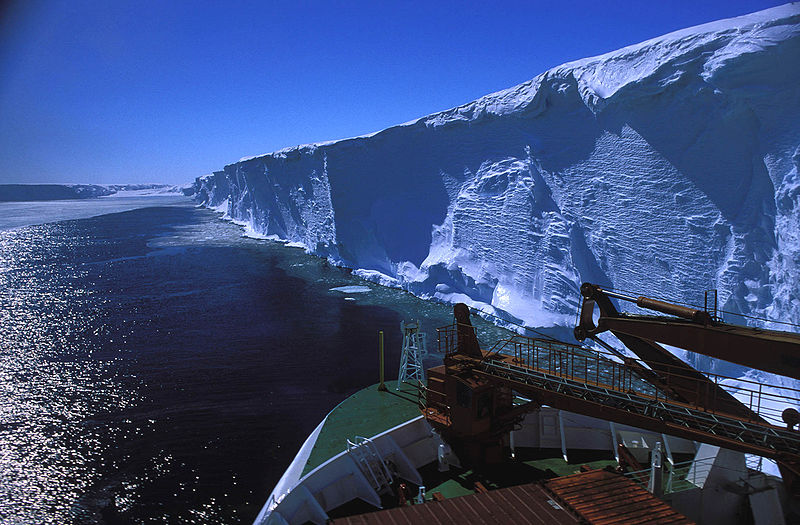
\includegraphics[width=0.6\textwidth]{iceshelfedge}

\tiny Ekstr\"om ice shelf(Hans Grobe)
\end{center}
\end{frame}


\begin{frame}{shallow shelf approximation stress balance 2}

SSA also applies reasonably well to \alert{ice streams}
\begin{itemize}
\item \dots with modest bed topography
\item \dots and weak bed strength\footnote{energy conservation (esp.~ice temperature and basal melt) and subglacial hydrology (esp.~subglacial water pressure) are major aspects of ice stream flow \dots but not addressed here}
\item imperfect near shear margins and grounding lines
\end{itemize}

\begin{center}
  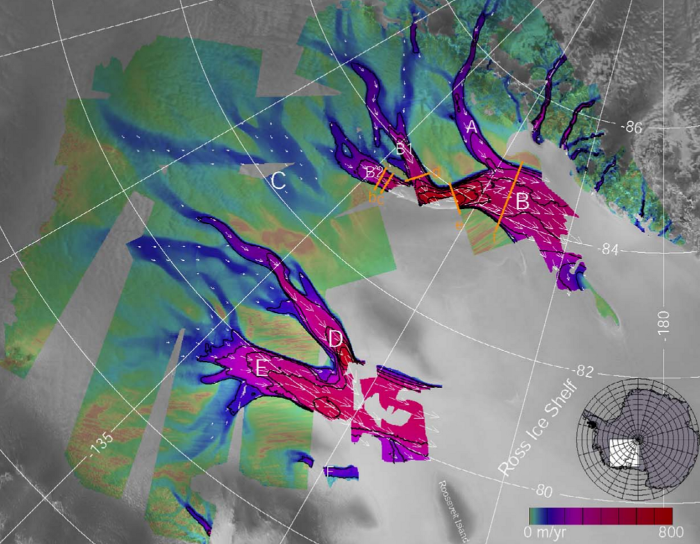
\includegraphics[width=0.6\textwidth]{siple}

\tiny surface velocity for Siple Coast ice streams, Antarctica 
\end{center}
\end{frame}


\begin{frame}{what is, \emph{and is not}, an ice stream?}

\begin{columns}
\begin{column}{0.6\textwidth}
\begin{itemize}
\item ice streams 
  \small
  \begin{itemize}
  \item[$\circ$] slide ($100$ to $1000 \,\text{m}\,\text{a}^{-1}$)
  \item[$\circ$] have concentrated vertical shear in thin layer near base
  \end{itemize}
  \normalsize
\item ``outlet glaciers''
  \begin{itemize}
  \item[$\circ$] fast surface speed (up to $10 \,\text{km}\,\text{a}^{-1}$)
  \item[$\circ$] uncertain how much is sliding
  \item[$\circ$] substantial vertical shear ``up'' in the ice column,
  \item[$\circ$] not-at-all flat bed topography
  \item[$\circ$] soft, temperate ice may play a big role
  \end{itemize} 
\item \alert{few simplifying assumptions are appropriate for outlet glaciers}
\end{itemize}
\end{column}

\begin{column}{0.4\textwidth}
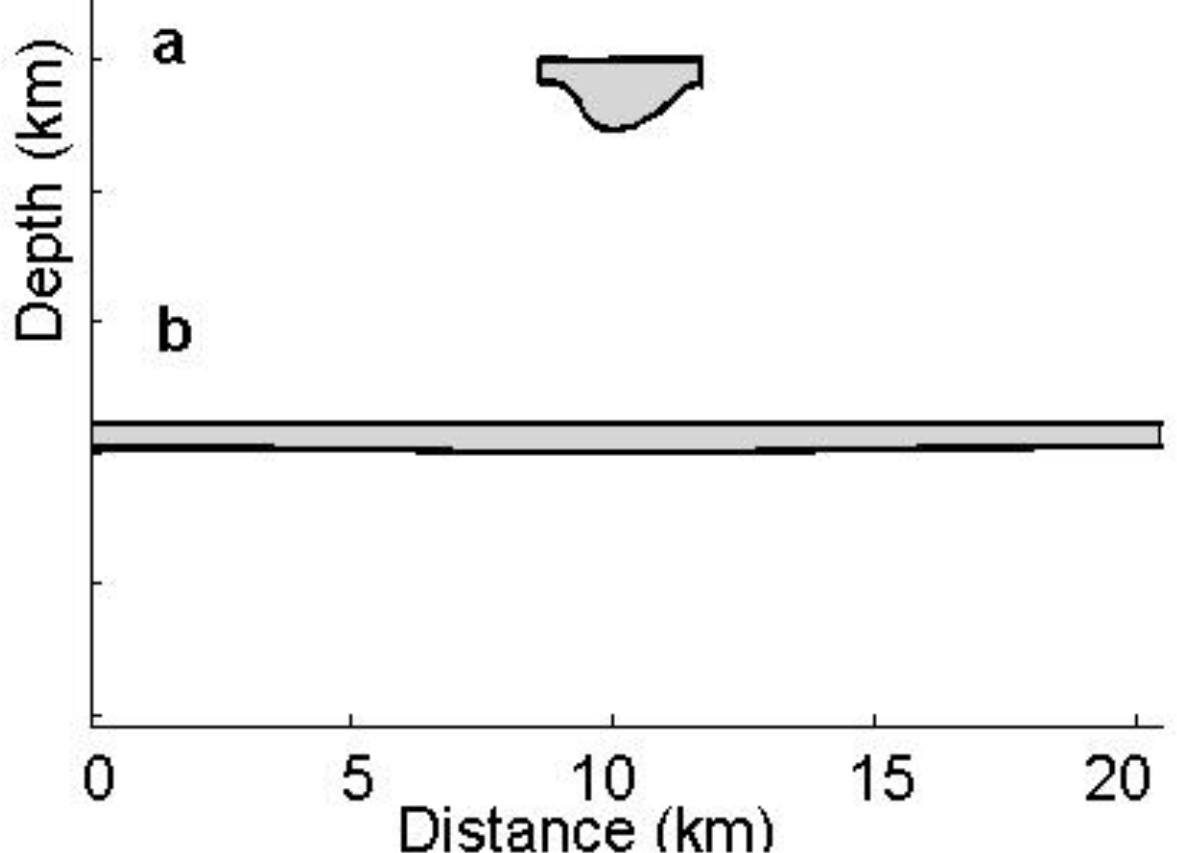
\includegraphics[width=1.0\textwidth]{streamisbrae}

\bigskip
\scriptsize 
Jakobshavns Isbrae (\textbf{a}) and Whillans Ice Stream (\textbf{b}); plotted without vertical exaggeration (\tiny Truffer and Echelmeyer (2003), \emph{Of isbrae and ice streams}\scriptsize \nocite{TrufferEchelmeyer})
\end{column}
\end{columns}
\end{frame}


\begin{frame}{SSA stress balance equation}

\begin{itemize}
\item only plane flow case (``flow line'') here
\item the stress balance equation which determines velocity in an \emph{ice stream}:
\begin{empheq}[box=\fbox]{equation}
  \left({\color{red}2 A^{-1/n} H |u_x|^{1/n - 1} u_x}\right)_x - {\color{blue}C|u|^{m-1}u} = {\color{green}\rho g H h_x} \label{ssa}
\end{empheq}
\item the {\color{red} red term} inside parentheses is the vertically-integrated ``longitudinal'' or ``membrane'' stress
\item the {\color{blue} blue term} is basal resistance
\item the {\color{green} green term} is  driving stress
\item derived originally by Morland (1987)\nocite{Morland}, MacAyeal (1989)\nocite{MacAyeal}
\item \emph{how to think about this equation}?
\item \emph{how do you solve it numerically}?
\end{itemize}
\end{frame}


\begin{frame}{flow line model: from stream to shelf}
\label{slide:streamtoshelf}

\small
\begin{align*}
  u = u_0 & \qquad \text{ at } x = 0 \\
  \left.\begin{array}{r}
  \left(2 A^{-1/n} H |u_x|^{1/n - 1} u_x\right)_x - C|u|^{m-1}u = \rho g H h_x \\
  h = H + b
  \end{array}\right\}& \qquad \text{ on } 0 < x < x_g \\
  \left.\begin{array}{r}
  \left(2 A^{-1/n} H |u_x|^{1/n - 1} u_x\right)_x + 0 = \rho g H h_x \\
  h = (1-\rho/\rho_w) H
  \end{array}\right\}& \qquad \text{ on } x_g < x < x_c \\
  2 A^{-1/n} H |u_x|^{1/n - 1} u_x = \frac{1}{2}\rho (1-\rho/\rho_w) g H^2 & \qquad \text{ at } x = x_c
\end{align*}

\bigskip\bigskip
\begin{center}
  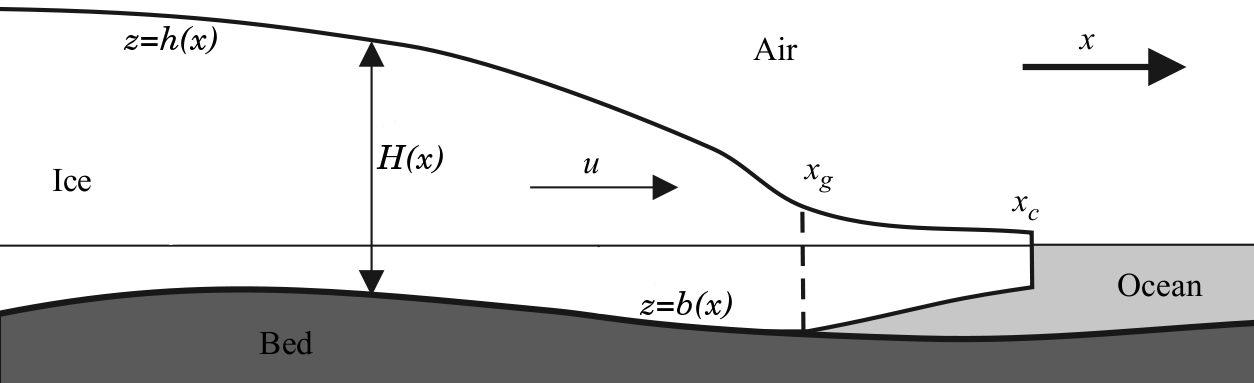
\includegraphics[width=0.7\textwidth]{flowline}
\end{center}
\end{frame}


\begin{frame}{flotation criterion and grounding line}

\begin{itemize}
\item the inequality ``$\rho H < - \rho_w b$'' is the \alert{flotation criterion}
\item at the grounding line $x=x_g$ the above inequality switches
\item \dots and the driving stress switches form:
  \begin{itemize}
  \item[$\circ$] on the grounded side we know $\rho H > - \rho_w b$ so
  	$$\rho g H h_x = \rho g H (H_x + b_x)$$
  \item[$\circ$] on the floating side we know $\rho H < - \rho_w b$ so $h = (1-\rho/\rho_w) H$ and so
  	$$\rho g H h_x = \rho(1-\rho/\rho_w) g H H_x$$
  \end{itemize}
\item also: $H,u,u_x$ are all continuous at $x=x_g$
\end{itemize}
\end{frame}



\subsection{ice shelf flow line solution}


\begin{frame}{exact velocity and thickness for steady ice shelf}

\begin{itemize}
\item limited goal here: describe a steady state, 1D ice shelf
\item there is a nice \alert{by-hand} result (next slide): the thickness and velocity in the ice shelf can be completely determined \nocite{MacAyealBarcilon,vanderVeen85} in terms of the 
  \begin{enumerate}
  \item ice thickness $H_g$ at the grounding line and
  \item ice velocity $u_g$ at the grounding line
  \end{enumerate}
\item we will use this to
  \begin{itemize}
  \item[$\circ$] understand the SSA better
  \item[$\circ$] verify a numerical SSA code
  \end{itemize}
\end{itemize}
\end{frame}


\begin{frame}{exact velocity and thickness for steady ice shelf 2}

\small see \texttt{testshelf.m} 

\begin{center}
  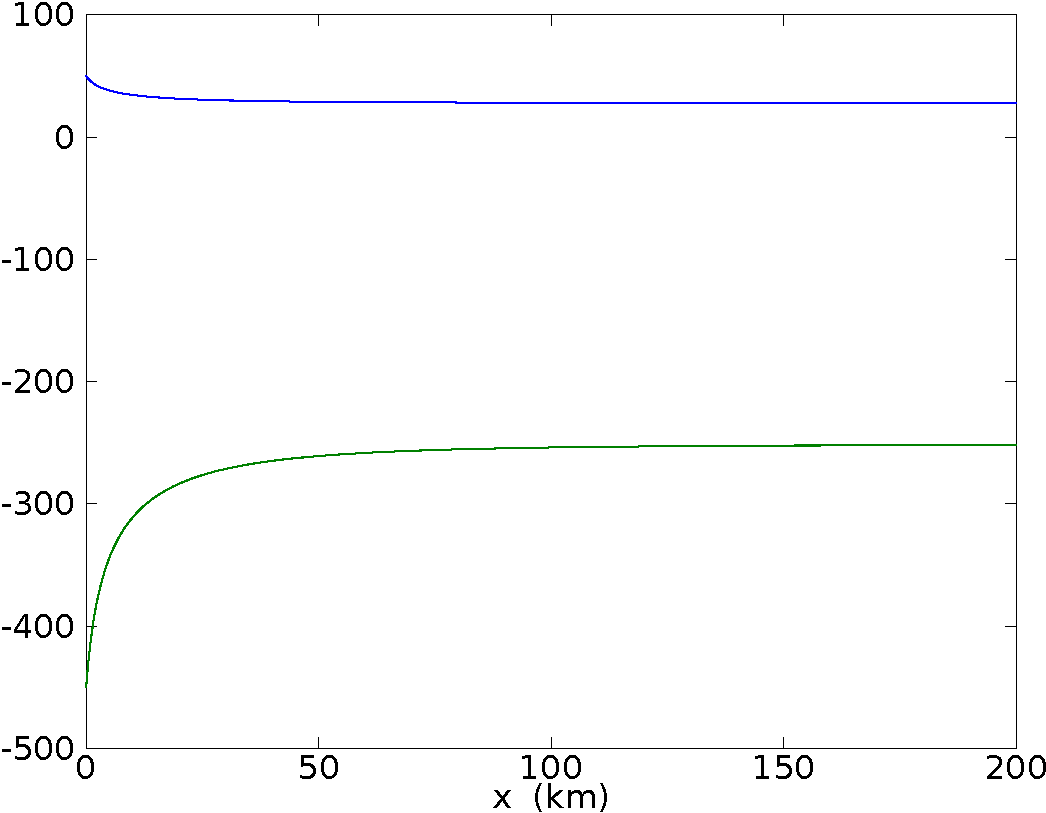
\includegraphics[width=0.45\textwidth]{steadyshelfprofile} \quad
  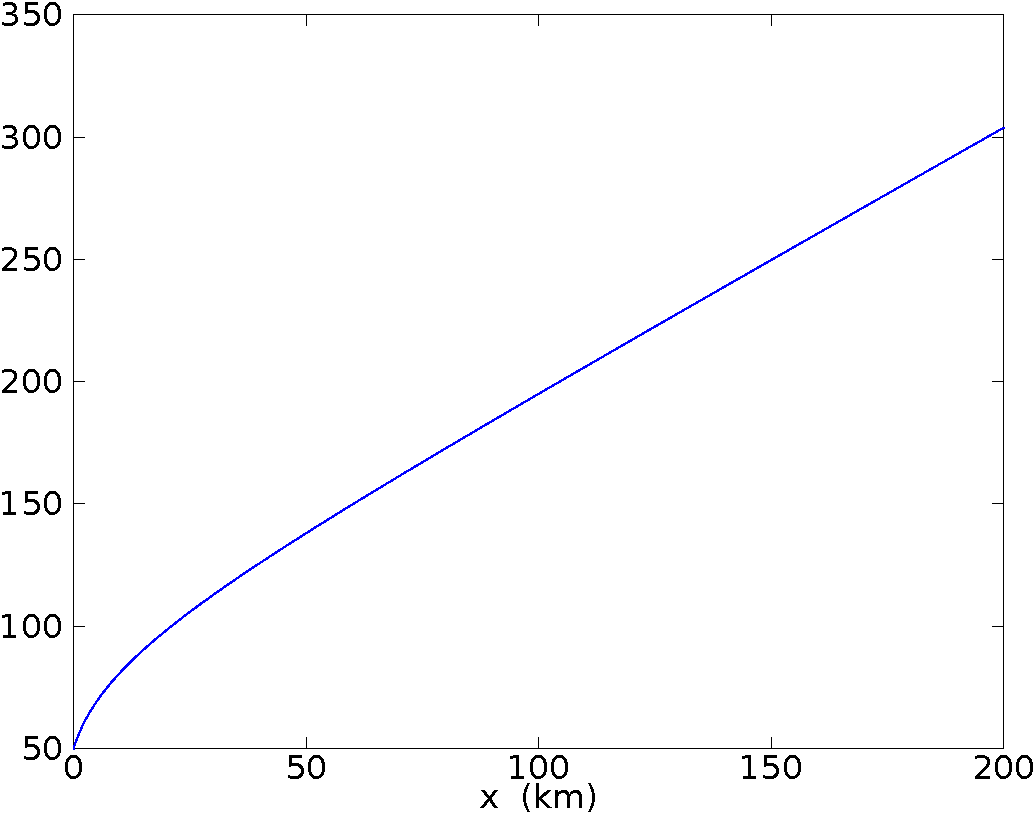
\includegraphics[width=0.45\textwidth]{steadyshelfvelocity}
\end{center}

\bigskip\bigskip
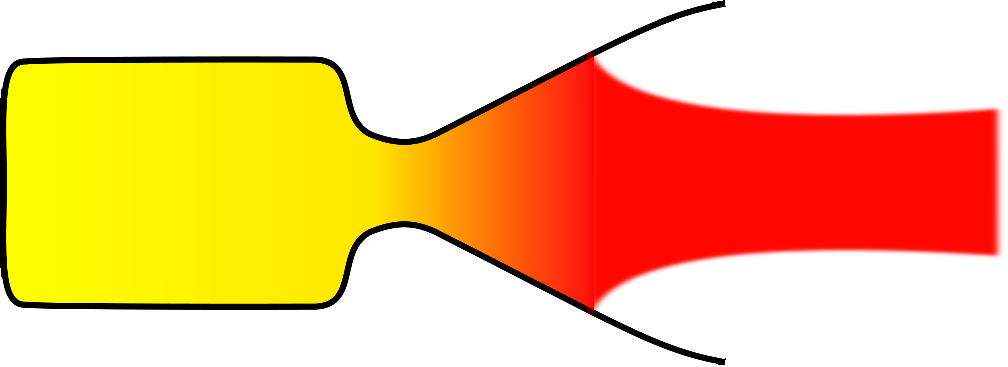
\includegraphics[width=0.3\textwidth]{rocket-nozzle-expansion}
\end{frame}


\subsection{numerical SSA}

\begin{frame}{numerically solving the SSA stress balance}

\begin{itemize}
\item here we fix ice thickness $H(x)$ and find the velocity numerically
\item the stress balance is a nonlinear equation in the velocity:
  $$\left(2 A^{-1/n} H |u_x|^{1/n - 1} u_x\right)_x - C|u|^{m-1}u = \rho g H h_x$$
\item \alert{iteration is needed}
\item I'll describe the numerical method for a shelf \emph{or} stream, but only give a code for an ice shelf
\end{itemize}
\end{frame}


\begin{frame}{numerically solving the SSA stress balance 2}

\begin{itemize}
\item coefficient ${\color{red} \bar \nu} = A^{-1/n} |u_x|^{1/n-1}$ is the ``effective viscosity'':
   $$\left(2 \,{\color{red} \bar \nu}\, H u_x\right)_x - C |u|^{m-1} u = \rho g H h_x$$
\item \emph{simplest iteration idea}: use old effective viscosity to get new velocity solution, and repeat until things stop changing
  \begin{itemize}
  \item[$\circ$] this is ``Picard'' iteration
  \item[$\circ$] Newton iteration is a superior alternative
  \end{itemize}
\item specifically:
  \begin{itemize}
  \item[$\circ$] last iterate $u^{(k-1)}$
  \item[$\circ$] define $W^{(k-1)} = 2 \bar \nu H = 2 A^{-1/n} |u^{(k-1)}_x|^{1/n-1} H$
  \item[$\circ$] current iterate (unknown) $u^{(k)}$
  \item[$\circ$] solve repeatedly:
     $$\left(W^{(k-1)} u^{(k)}_x\right)_x - C |u^{(k-1)}|^{m-1} u^{(k)} = \rho g H h_x$$
  \end{itemize}
\end{itemize}
\end{frame}


\begin{frame}{solving the ``inner'' linear problem}
\begin{itemize}
\item abstract the problem:
   $$\left(W(x)\, u_x\right)_x - \alpha(x)\, u = \beta(x)$$
on $0 < x < L$, with boundary conditions
   $$u(0) = V, \qquad  u_x(L) = \gamma$$
\item an \emph{elliptic} PDE boundary value problem
\item $W(x)$, $\alpha(x)$, $\beta(x)$ are known functions in the SSA context:
  \begin{itemize}
  \item[$\circ$] both $W(x)$ and $\alpha(x)$ come from previous iteration
  \item[$\circ$] $\beta(x)$ is driving stress
  \end{itemize}
\end{itemize}
\end{frame}


\begin{frame}{where do you get an initial guess $u^{(0)}$?}

\begin{itemize}
\item \emph{for floating ice}, a possible initial guess for velocity comes from assuming a uniform strain rate:
   $$u^{(0)}(x) = \gamma (x-x_g) + u_g$$
where $\gamma$ is the value of $u_x$ found from calving front stress imbalance
\item \emph{for grounded ice}, a possible initial guess for velocity is to assume ice is held by basal resistance only:
   $$u^{(0)}(x) = \left(-C^{-1} \rho g H h_x\right)^{1/m}$$
\end{itemize}
\end{frame}


\begin{frame}{numerics of the ``inner'' linear problem}

\begin{itemize}
\item suppose $j=1,2,\dots,J+1$, where $x_1 = x_g$ and $x_{J+1} = x_c$ are endpoints
\item $W(x)$ is needed on the staggered grid; the approximation is:
$$\frac{W_{j+1/2} (u_{j+1} - u_j) - W_{j-1/2} (u_{j} - u_{j-1})}{\Delta x^2} - \alpha_j u_j \stackrel{\ast}{=} \beta_j$$
\item left-hand boundary condition: $u_1 = V$ given
\item right-hand boundary condition (``$u_x(L)=\gamma$''):
  \begin{itemize}
  \item[$\circ$] introduce notional point $x_{J+2}$
  \item[$\circ$]
    $$\frac{u_{J+2} - u_J}{2 \Delta x} = \gamma$$
  \item[$\circ$] using equation $\ast$ in $j=J+1$ case, eliminate $u_{J+2}$ variable ``by-hand'' before coding numerics \nocite{MortonMayers}
  \end{itemize}
\end{itemize}
\end{frame}


\begin{frame}{numerics of the ``inner'' linear problem 2}

\scriptsize
\begin{itemize}
\item so SSA stress balance has form  \quad $A \mathbf{x} = \mathbf{b}$, \quad namely:
$$
\begin{bmatrix}
1 &  &  &  &  \\
W_{3/2} & A_{22} & W_{5/2} &  &  \\
 & W_{5/2} & A_{33} &  &  \\
 &  & \ddots & \ddots &  \\
 &  & W_{J-1/2} & A_{JJ} & W_{J+1/2} \\
 &  &  & A_{J+1,J} & A_{J+1,J+1} \\
\end{bmatrix}\,
\begin{bmatrix}
u_1 \\ u_2 \\ u_3 \\ \vdots \\ u_J \\ u_{J+1}
\end{bmatrix}
=
\begin{bmatrix}
0 \\ \beta_2 \Delta x^2 \\ \beta_3 \Delta x^2 \\ \vdots \\ \beta_J \Delta x^2 \\ b_{J+1}
\end{bmatrix}
$$
\item with diagonal entries
$$A_{22} = -(W_{3/2}+W_{5/2}+\alpha_1 \Delta x^2)$$
$$A_{33} = -(W_{5/2}+W_{7/2}+\alpha_2 \Delta x^2)$$
and so on, up to $A_{JJ}$, 
\item with special cases in last equation:
$$A_{J+1,J} = 2 W_{J+1/2}$$
$$A_{J+1,J+1} = -(2 W_{J+1/2}+\alpha_{J+1}\Delta x^2)$$
$$b_{J+1} = -2 \gamma \Delta x W_{J+3/2} + \beta_{J+1} \Delta x^2$$
\item this is a \emph{tridiagonal} system
\end{itemize}
\end{frame}


\begin{frame}{numerics of the ``inner'' linear problem 3}
\label{slide:flowlinecode}

\minput{flowline}
\end{frame}


\begin{frame}{testing the ``inner'' linear code}

\begin{itemize}
\item before proceeding to solve nonlinear SSA problem, we can test the ``abstracted'' code \texttt{flowline.m}
\item test by ``manufacturing'' solutions
  \begin{itemize}
  \item[$\circ$] see \texttt{testflowline.m}; not shown
  \end{itemize}
\item results:
  \begin{itemize}
  \item[$\circ$] converges at optimal rate $O(\Delta x^2)$
  \end{itemize}
\end{itemize}
\end{frame}


\begin{frame}{numerical: SSA}

\minputtiny{ssaflowline}
\end{frame}


\begin{frame}[fragile]
  \frametitle{\emph{numerical} thickness and velocity for steady ice shelf}

lines below are a convergence analysis of \texttt{testshelf.m}, which calls \texttt{ssaflowline.m}:

\begin{center}
  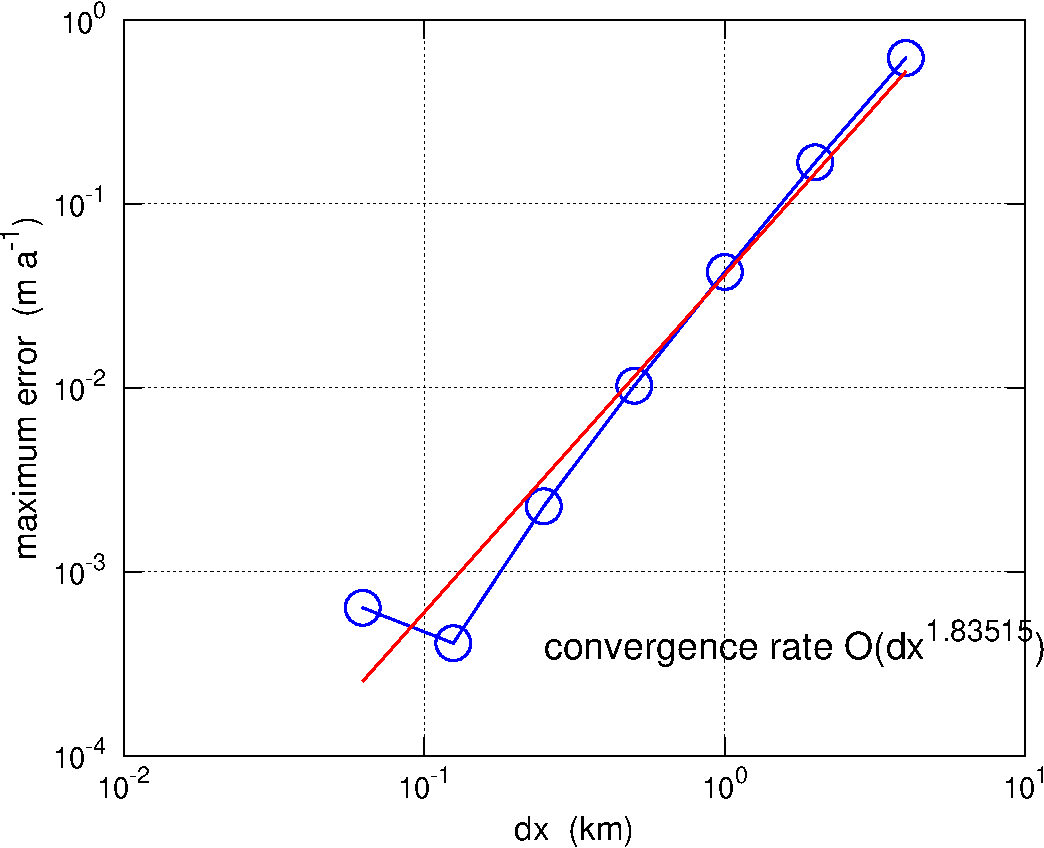
\includegraphics[width=0.75\textwidth]{shelfconv}
\end{center}
\end{frame}


\begin{frame}{SSA model output}

\begin{center}
  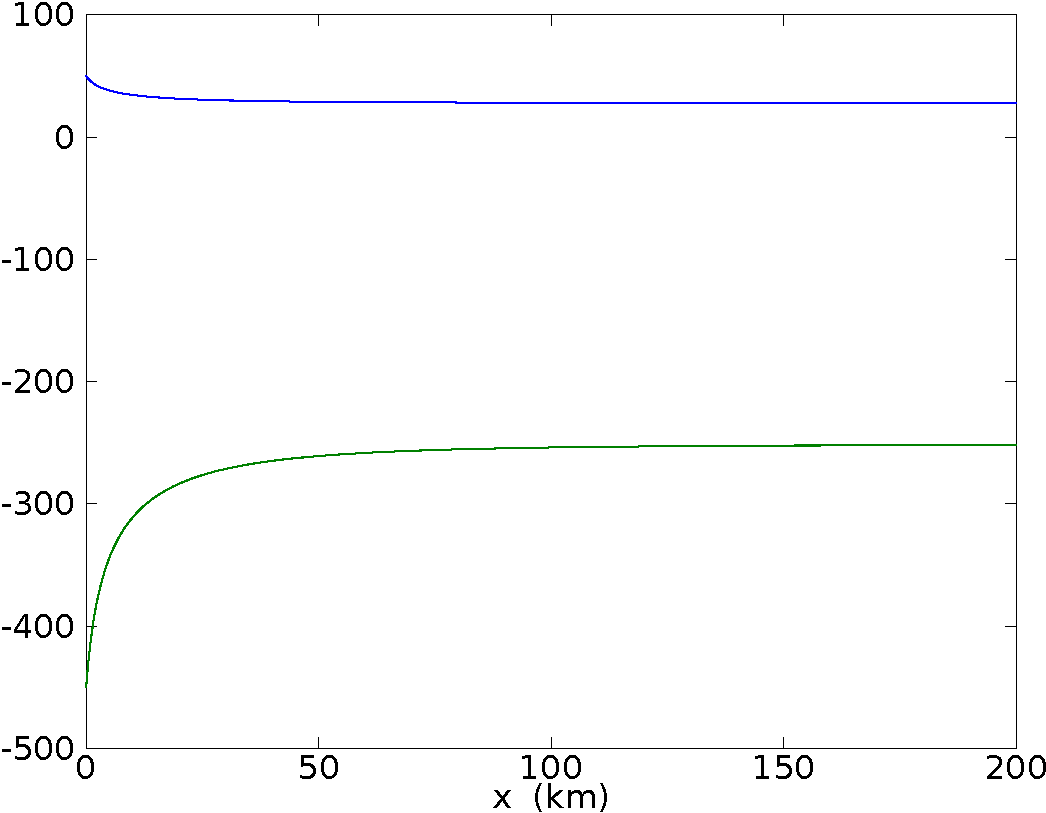
\includegraphics[width=0.45\textwidth]{steadyshelfprofile} \quad
  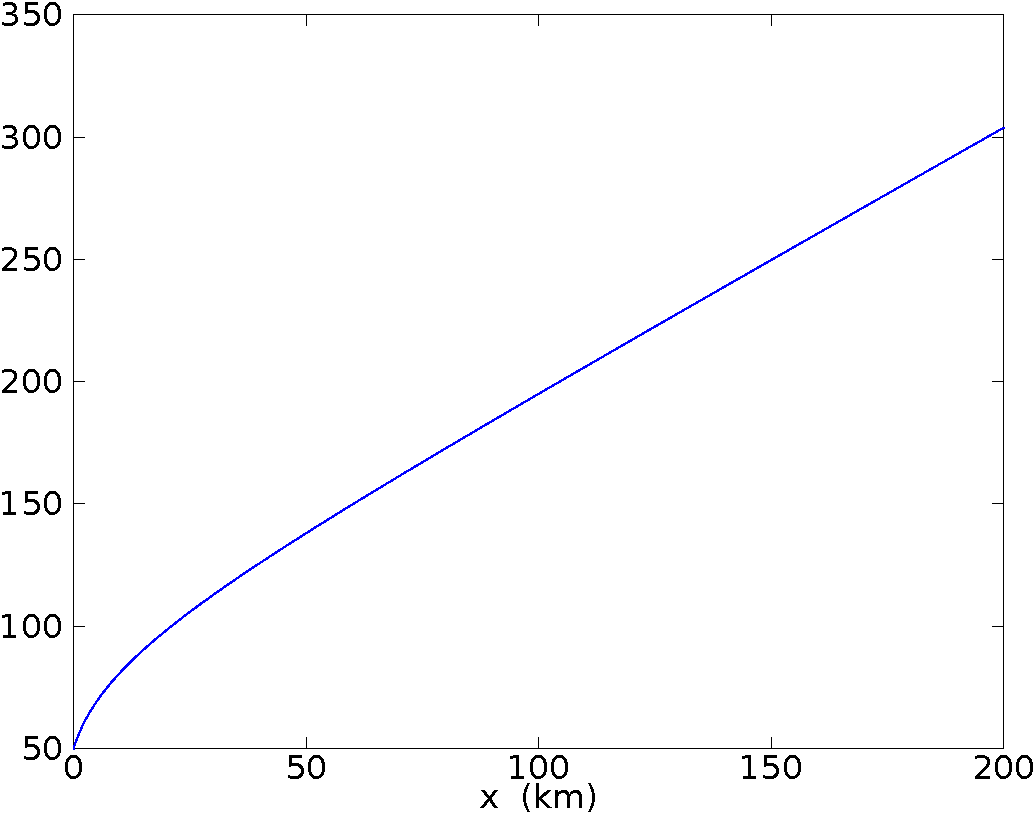
\includegraphics[width=0.45\textwidth]{steadyshelfvelocity}
\end{center}

\bigskip

\begin{itemize}
\item \emph{this looks suspiciously like figures for the exact solution \dots}
\item yes
\end{itemize}
\end{frame}


\begin{frame}{realistic ice shelf modeling}

\begin{itemize}
\item flow lines are never very realistic
\item you can add parameterized ``side drag'' \dots
\item also, ice shelves have surprises:
  \begin{itemize}
  \item[$\circ$] high basal melt near grounding lines
  \item[$\circ$] marine ice can freeze-on at bottom (below)
  \item[$\circ$] ``reverse slope'' bed instability and WAIS \dots
  \end{itemize}
\end{itemize}

\medskip
\begin{center}
  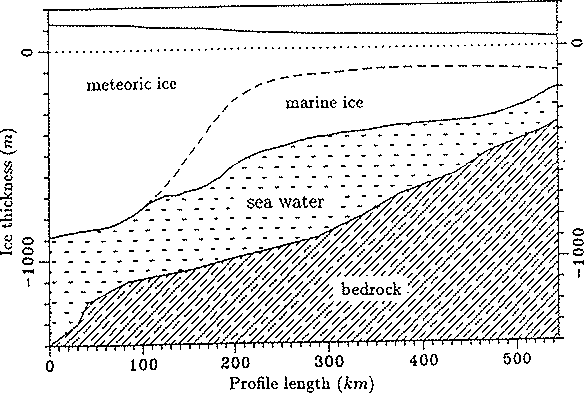
\includegraphics[width=0.5\textwidth]{marineice}
  
  \medskip
  \tiny from Grosfeld \& Thyssen 1994 \nocite{GrosfeldThyssen1994}
\end{center}
\end{frame}


\begin{frame}{ice shelf modeling in 2D}

\begin{itemize}
\item nonetheless ``diagnostic'' (static geometry) ice shelf modeling in 2d has been quite successful
\item observed surface velocities validate SSA stress balance model
  \begin{itemize}
  \item[$\circ$] e.g.~Ross ice shelf example below using PISM
  \item[$\circ$] \dots but many models can do this
  \end{itemize}
\end{itemize}

\begin{center}
  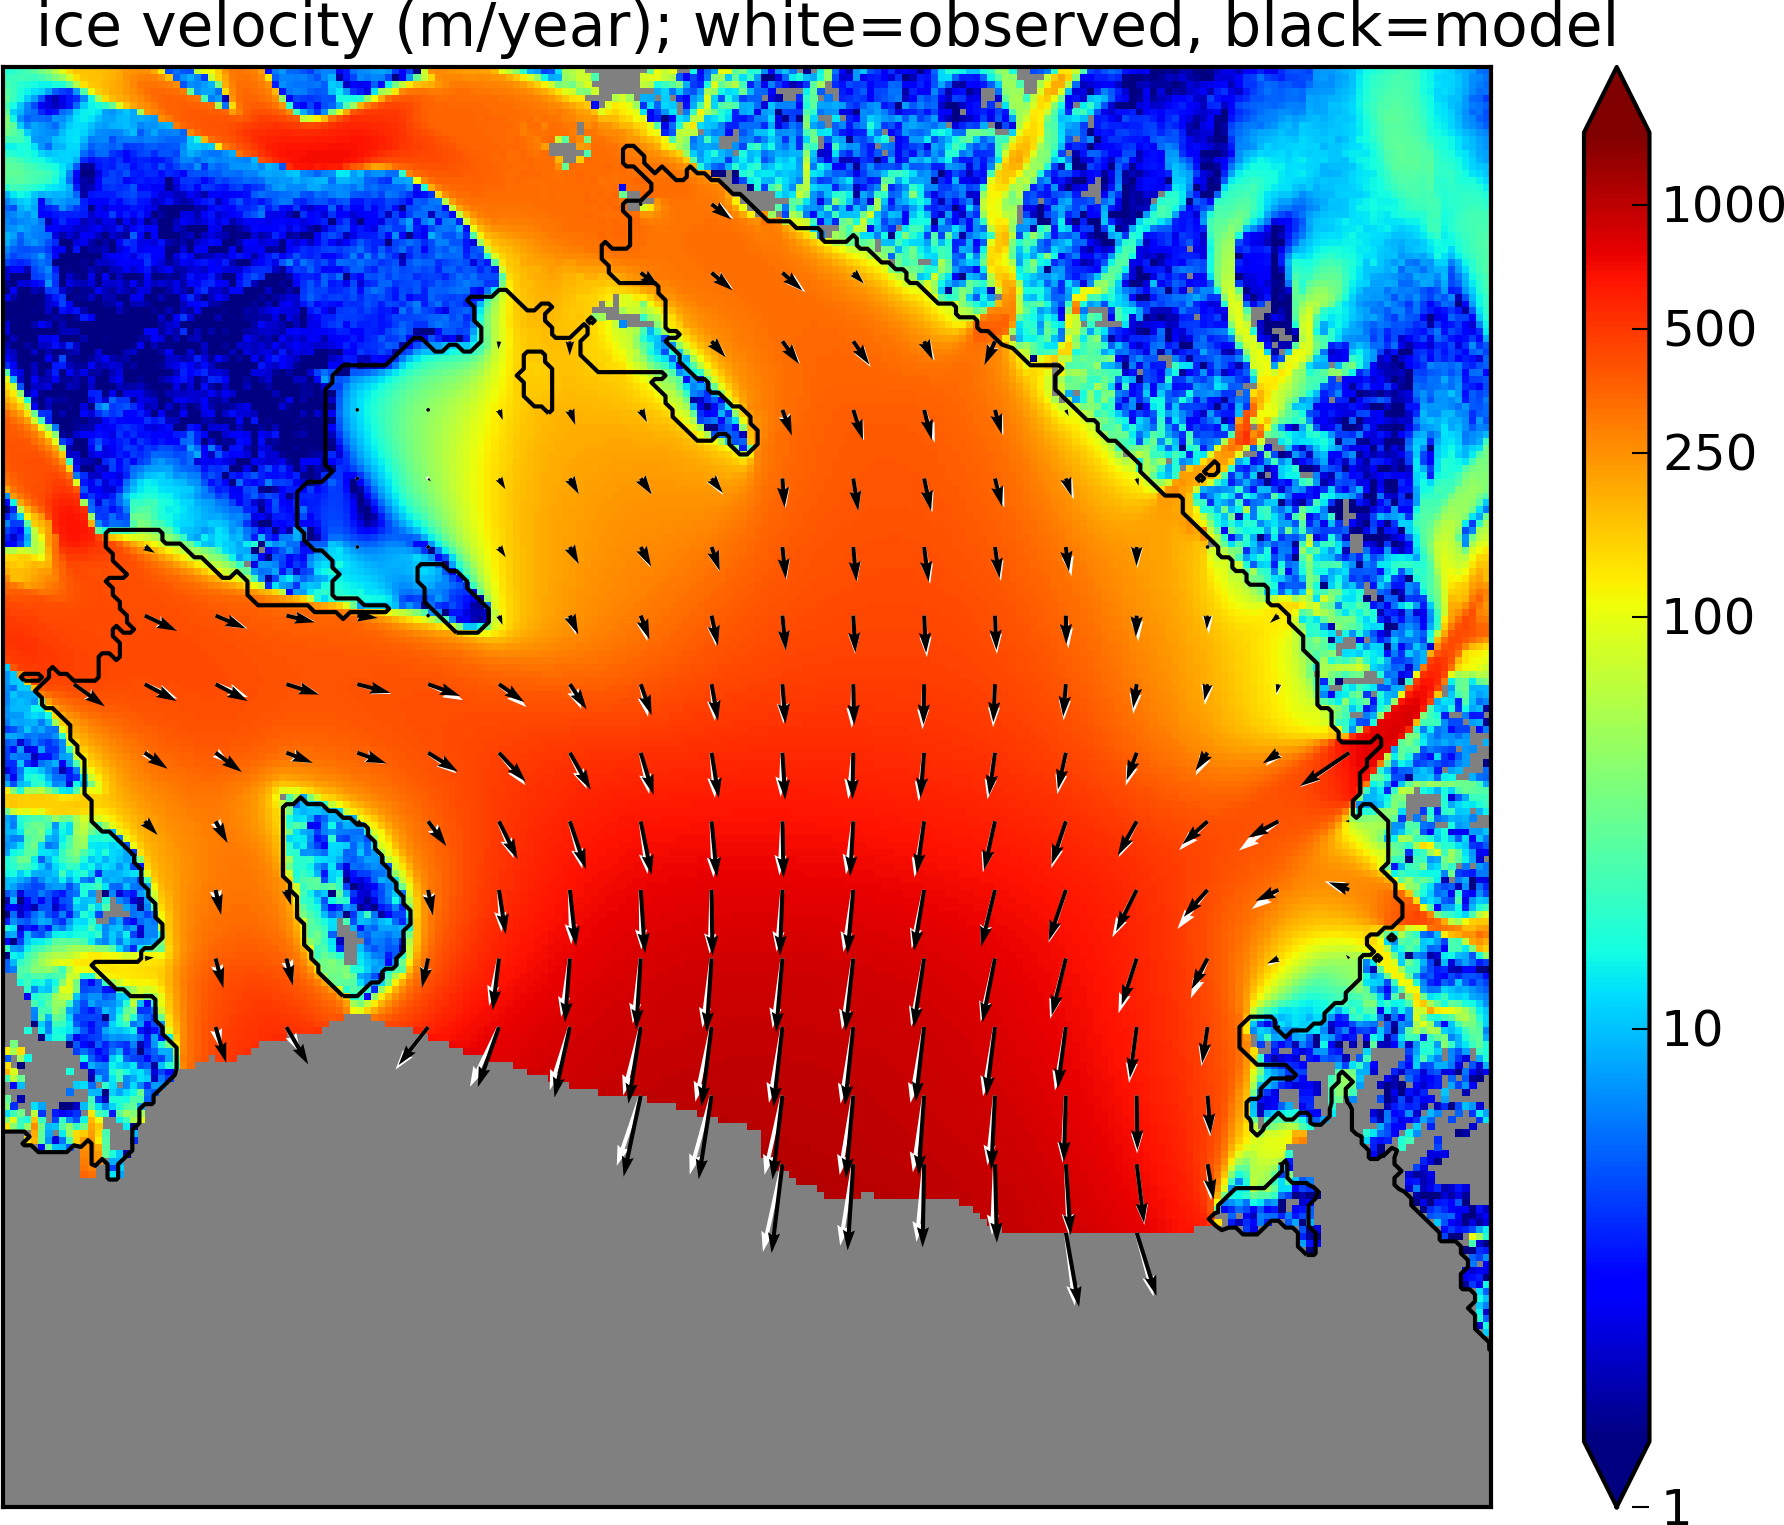
\includegraphics[width=0.5\textwidth]{rossquiver} \quad  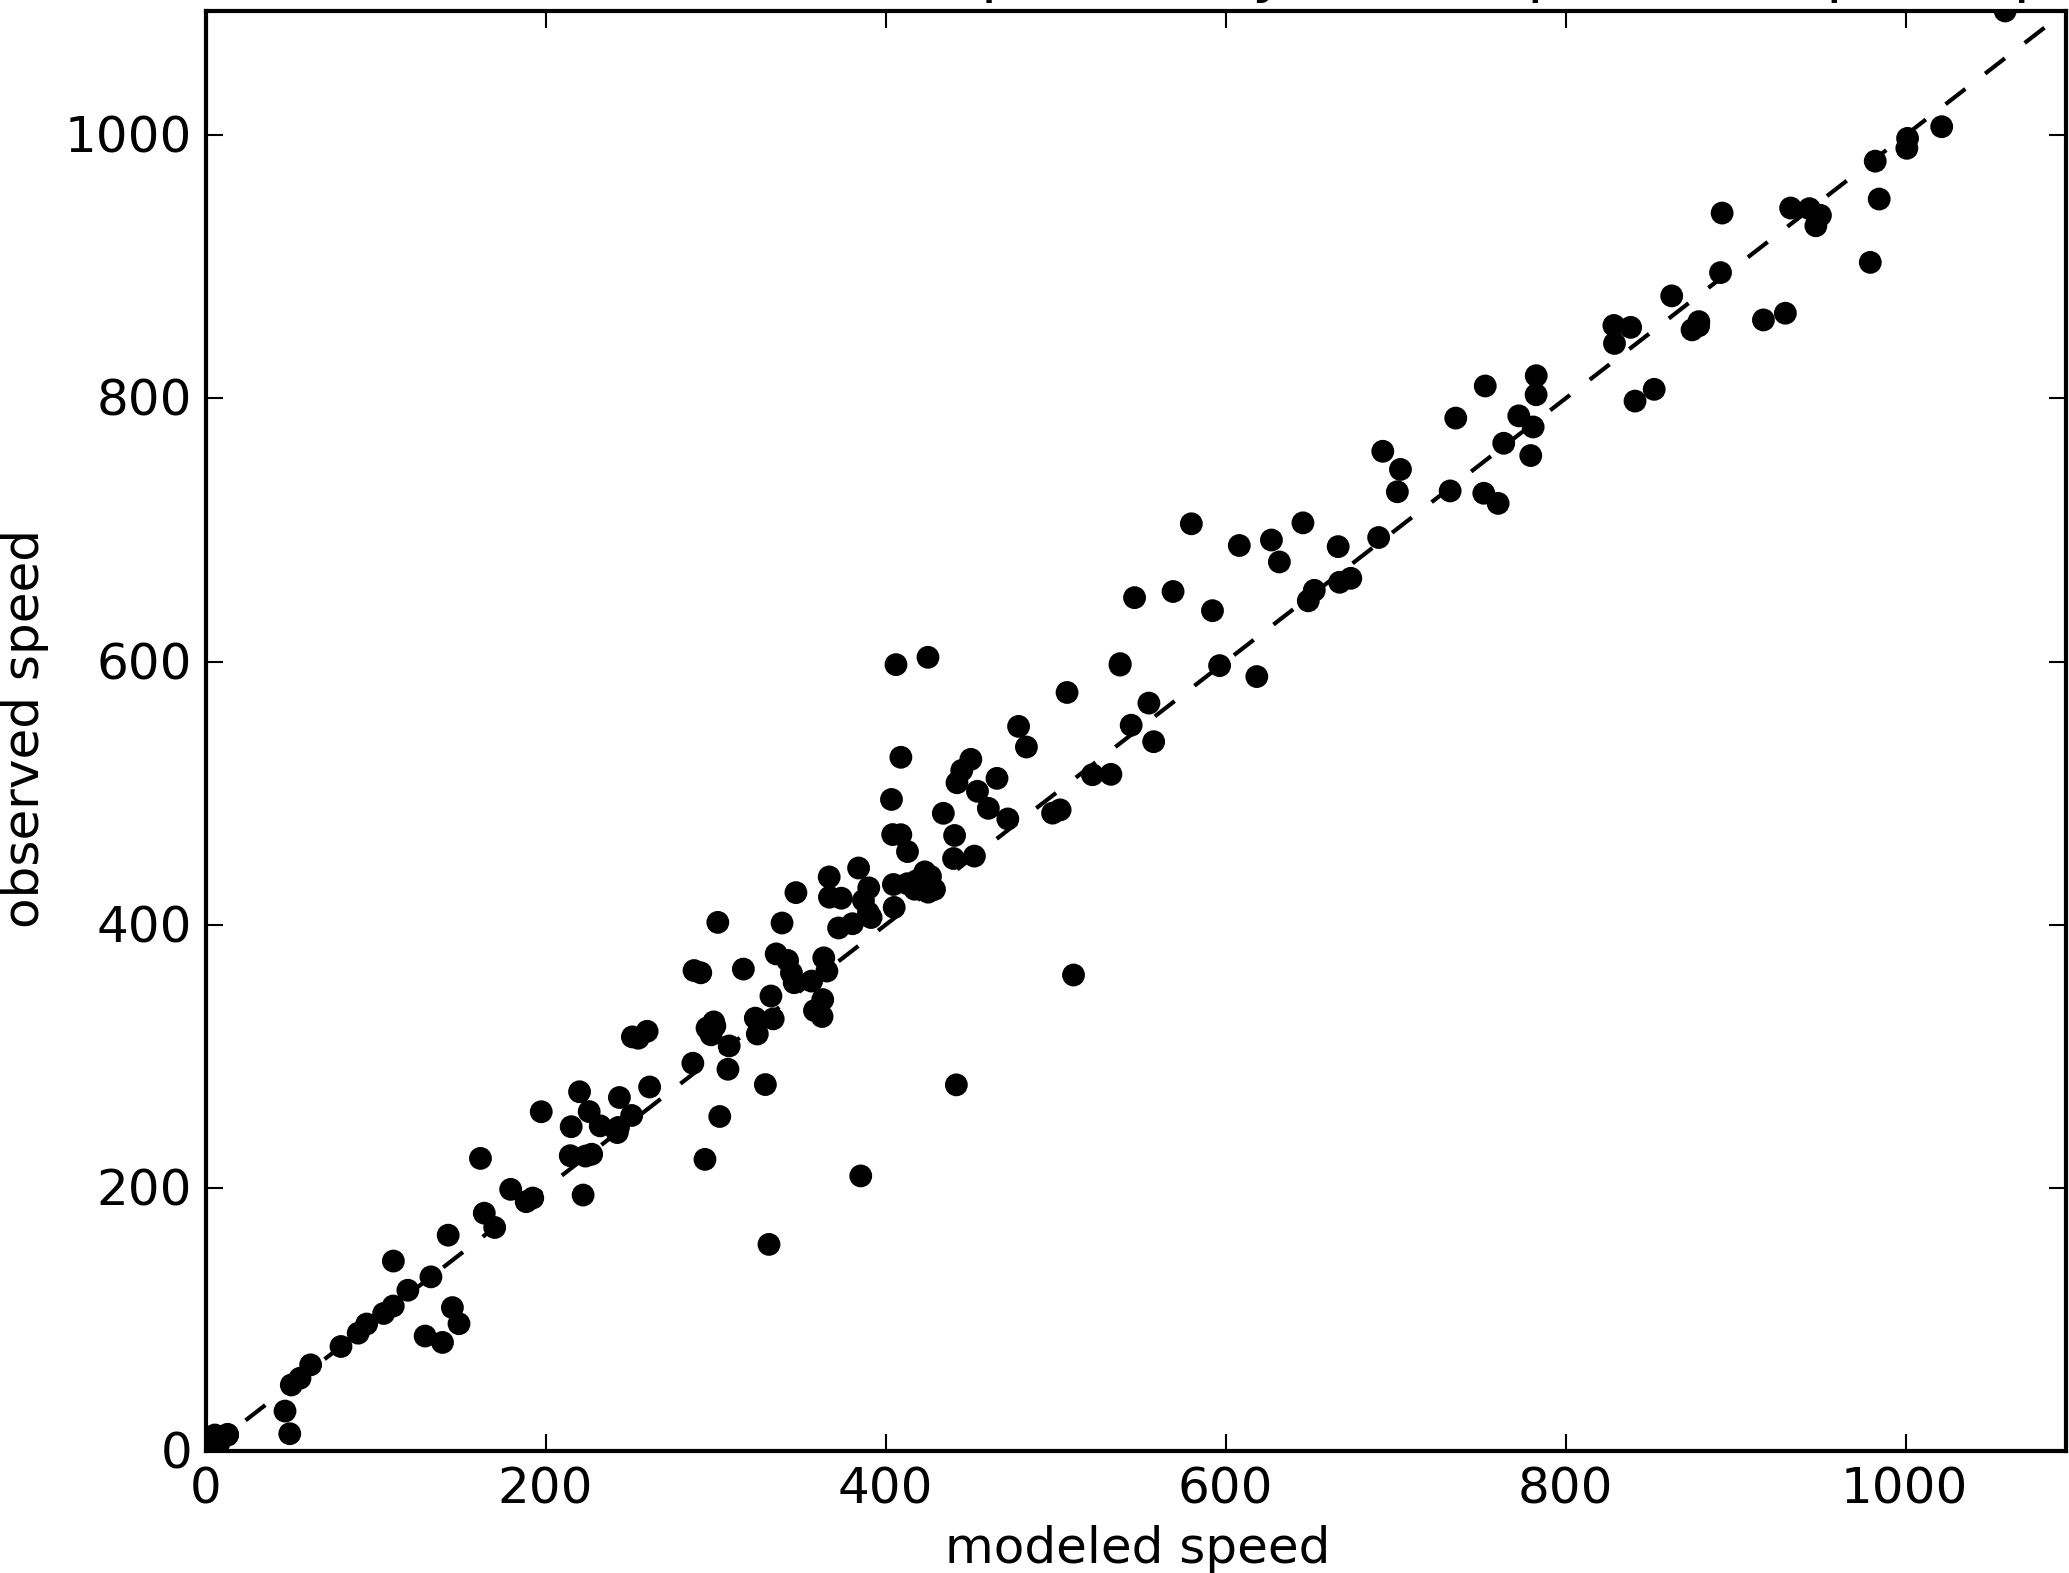
\includegraphics[width=0.45\textwidth]{rossscatter}
\end{center}
\end{frame}


\begin{frame}{numerical solution of stress balances: a summary}

\begin{itemize}
\item stress balance equations (e.g.~SSA or Stokes) determine velocity from geometry and boundary conditions
  \begin{itemize}
  \item[$\circ$] nonlinear so iteration is necessary
  \item[$\circ$] at each iteration a sparse matrix ``inner'' problem is solved \dots give it to a matrix solver software package
  \end{itemize}

\bigskip
\item general principles:
  \begin{itemize}
  \item[$\circ$] \alert{modularize your code}
  \item[$\circ$] \alert{test the parts}
  \end{itemize}
\end{itemize}
\end{frame}


\begin{frame}{the mass continuity equation: a summary}

\begin{itemize}
\item the \emph{mass continuity equation} is
  $$H_t = M - \nabla \cdot (\mathbf{u} H)$$
\item the numerical nature of this equation depends on the stress balance:
  \begin{itemize}
  \item[$\circ$] the equation is a diffusion for frozen bed, large scale flows (i.e.~SIA)
  \item[$\circ$] it is \emph{not} very diffusive for membrane stresses and no basal resistance (e.g.~SSA for ice shelves)
  \item[$\circ$] it is diffusive for ice streams (but how much?)
  \item[$\circ$] there is \emph{not} much helpful theory on this transport problem
  \item[$\circ$] \dots maybe you will help find this theory!
  \end{itemize}
\end{itemize}
\end{frame}

